\documentclass[letterpaper,twocolumn,10pt]{article}
\usepackage{usenix,epsfig,endnotes}
\usepackage{graphicx, amsfonts, amsmath, amsthm, wrapfig, color}
\usepackage{hyperref}
\usepackage[parfill]{parskip}
\usepackage{fullpage}

\newcommand{\includeimage}[2] {\fbox{ \includegraphics[width=#1]{#2}}}
 
\begin{document}

%don't want date printed
\date{}

%make title bold and 14 pt font (Latex default is non-bold, 16 pt)
\title{\Large \bf A Real-time Hand Gesture Recognition System}

%for single author (just remove % characters)
\author{
{\rm Arun Ganesan}\\
University of Michigan, Ann Arbor
\and
{\rm Caoxie (Michael) Zhang}\\
University of Michigan, Ann Arbor
% copy the following lines to add more authors
% \and
% {\rm Name}\\
%Name Institution
} % end author

\maketitle

% Use the following at camera-ready time to suppress page numbers.
% Comment it out when you first submit the paper for review.
\thispagestyle{empty}

\begin{abstract}
Hello World
\end{abstract}

\section{Introduction}
Natural user interface (NUI) is a new way for human to interactive with machines. Among numerous NUIs which include multi-touch screen, eye tracking and many others, hand gesture seems to be one promising candidate. In this paper, we design and evaluate a novel hand gesture recognition system to demonstrate that we are close to an actual production-level system. The reader should be noticed that we do not claim hand gesture is THE future user interface, and in fact there are some limitations for using hand gestures such as users may feel fatigues (in the movie Minority Report, Tom Cruise has to take breaks many time due to fatigue). Similar to many other new UI systems, we propose our system as one (interesting) way to interact with the computer. We do not claim that the system would replace mouse and keyboard and we leave the usability problem to future research as building hand gesture recognition system alone is quite challenging. 


\subsection{Design Goals}
Our system is designed to maximize user experience. Moreover, our system differs from other existing systems in the following ways.

\textbf{Just hands.} The users do not need to attach any additional physical objects to use our systems. They just need to show up their hands. Many existing system such as [SixSense, MIT Minority Report, MIT color glove] require users to wear gloves or markers  for the RGB camera to capture. We eliminate this since the user should not do anything more than showing their hands. 
  
\textbf{Real-time.} Our system should run smoothly on a modern machine with a graphical card not just on high-end machines. The system should also recognize hand gesture at a high frame rate. Our desired frame rate 30Hz, although the current version has around 5Hz. In our design and implementation, one driving goal is to squeeze every milliseconds as possible. 

\textbf{No calibration.} Our system should not require a new user to do anything to calibrate the system to be used to the user. 

\textbf{Robust and Accurate.} Our system should have an accurate estimation of where the users' hands are and what gestures they use with low false positive. Moreover, the system should be insensitive to various background, user's location, camera position and other noise. 
  
\textbf{Arbitrary gestures.} Our system should be able to easily incorporate new types of gestures that any developers would like to add. By training new gestures, the system can recognize arbitrary gestures, for example the American sign language. 

\subsection{Main Ideas}
Our system would not be possible without the use of Microsoft Kinect for PC, which we are probably among the first to obtain it in February 2012. Kinect is a multi-purpose sensor including RGB camera, depth camera and audio sensor. The Kinect SDK has offered skeletal recognition, which is however far away from recognizing hand gesture. The SDK also provides raw pixels for the RGB image and depth image at a maximum frame rate 30Hz. We use the depth image for gesture recognition and both RGB and depth image for generating training samples. The depth image is the key factor that distinguishes our system from most existing systems that use RGB camera. The advantage of the depth image is that it offers an addition dimension, i.e. depth of each pixel that is not present in the RGB image. An illustrating example would be an object and its background has similar color but the depth of the two is drastically different. 

Our system adopts a data-driven approach: machine learning as opposed to hand-crafted rule-based systems. The adoption of machine learning transfers the human intelligent efforts from design rules/algorithms to design informative features. With the features on labeled data, machine learning allows computers to learn the rule/algorithm automatically. The key advantages of using machine learning in our system    
are (1) easy to incorporate developer-defined gestures: developers just need to feed the system with the gesture images to be trained rather than deriving new algorithms (2) robust to various environments such as camera position, background, various size of the hands: developers just need to generate the gestures on various environments without worrying about anything more. 

In a high-level overview, the system is separated into two parts: training and real-time prediction. Only the real-time prediction component is seen by the end users. In the training component, we use color gloves to generate massive labeled data of the depth image. Random forest is trained to achieve both real-time performance and high accuracy. In the real-time prediction component, each pixel in the depth image is predicted the type of the gesture using GPU and then the prediction outputs are pooled to propose the final position and type of a gesture. Notice that we do not use any temporal or kinetics information as the current simple design suffices for the hand gesture tracking.   [Need to elaborate more?] 



\subsection{Contributions}

We summarize our contributions as follows:

\textbf{A system for real-time hand gesture recognition.} We design and implement a complete real-time hand gesture recognition system based on machine learning. The system can be used as API for other applications to read the gesture in real-time.

\textbf{An inexpensive way to generate labeled data.} We color gloves to easily generate labeled data through the use of alignment of RGB and depth images. In [MSR], the authors use sophisticated computer graphics to generate training samples. We found this expensive and through the use of color gloves, developers can generate their customized gesture without difficulty. Notice that the end users do not need to wear any color gloves. 

\textbf{An computational insight about random forest and support vector machine (SVM).} To the best of our knowledge, there seems to be no literature in comparing  SVM and random forest from a computational perspective. We provide an in-depth comparison in the angle of performance rather than merely predictability as done in most machine learning literature. 

\textbf{Extensive experimental evaluations of the system.} We conduct extensive experiments evaluation on the effectiveness of the machine learning approach, i.e., random forest we use in a large space of parameters. Interesting results reveals a deeper understanding of random forest. 

Our work is made public at: \url{https://github.com/arunganesan/hand-gesture-recognition}.

\section{System Overview}
\label{sec: system}
\cutsection

The system architecture is visualized in Figure~\ref{fig: architecture}. From the user point of view, our system is divided into two components: developers mode for training gestures and end-user mode for real-time prediction. In a high-level overview, developers using the developer mode supply the system with labeled data with color gloves. The system trains with this labeled data. In the end-user mode, the camera captures raw depth images of the user's naked hands. It then predicts every pixel using the GPU and then pools the predicted pixels to get an estimation of the location of the gesture. Between the two modes, they share a component: feature extraction, which obtains the features for each pixel in the depth image. The implementation of feature extraction in the two modes are different - the training component uses the CPU in an off-line fashion and the end-user prediction component uses the GPU (end-user mode) in an on-demand fashion. 
\cutequation
\begin{figure}
\centering
	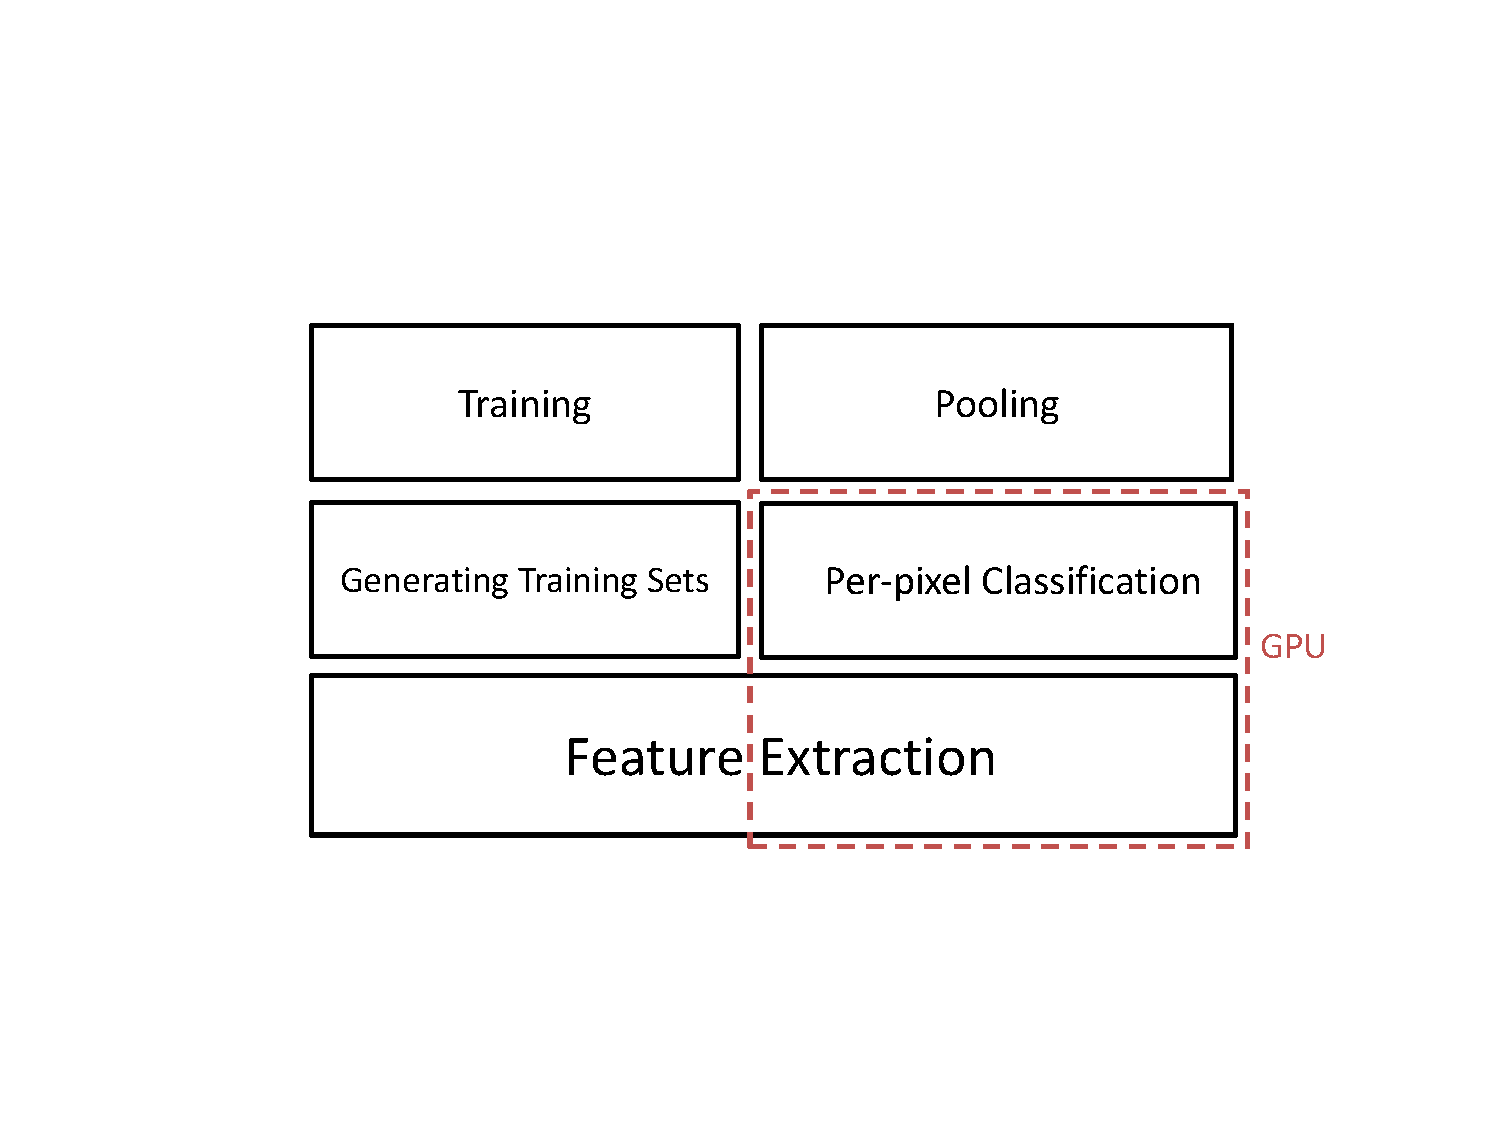
\includegraphics[width=0.5\textwidth]{fig/SystemArchitecture.pdf}
	\cutcaption
	\caption{An overview of the system architecture}
    \label{fig: architecture}
\end{figure}
\cutequation

\cutsection
\subsection{The Kinect Sensor}
\cutsection

The Kinect sensor provides both raw depth image and color image at a maximum frame rate of 30Hz and at 640px $\times$ 480px resolution. Each pixel in the depth image represent the distance from the object to the camera. The error of the depth can be with several millimeters. However, objects can have a shadow where some parts near the object do not have depth value at all. This is an example of realistic noise that may be missing if the training data was generated using computer graphics methods.

\section{Feature Extraction and Per-pixel Classification}
\label{sec: Classification}

In this section, we describe the main classification algorithm used in the system. At each frame, the system looks at the depth image, and predicts each pixel's type of gestures (e.g., open hand, close hand or background). The prediction result on every pixel will be fed into a pooling stage to propose the final gesture location and type. The driving reason for us to choose per-pixel classification is that it allows massive parallelism using GPU since each pixel is using the same predicting algorithm.  

\subsection{Feature Extractions}
\label{sec: feacture_extraction}
For each pixel \textbf{x}, we extract a group of features. Each group say $\theta=\{\bf{u}, \bf{v} \}$ corresponds to the depth difference between two points offset from \textbf{x} normalized by its depth:

\begin{align} 
\label{eqn:feature}
f_{\theta}(x) = d\left(\textbf{x} + \frac{\textbf{u}}{d(\textbf{x})}\right) - d\left(\textbf{x} + \frac{\textbf{v}}{d(\textbf{x})}\right)
\end{align}

\begin{figure}
	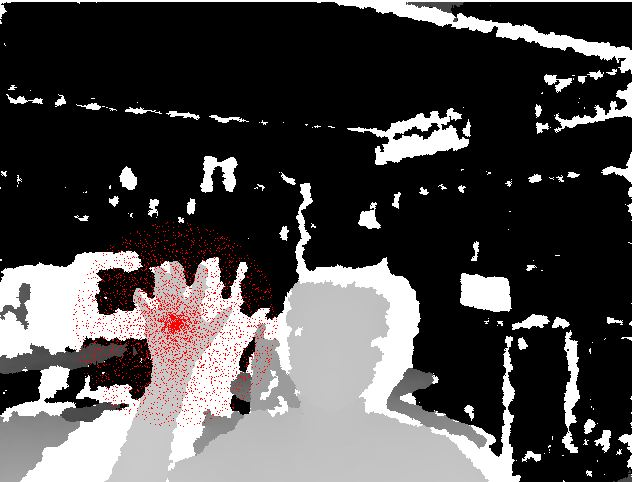
\includegraphics[width=0.23\textwidth]{fig/OpenHandNearOffset.jpg}
	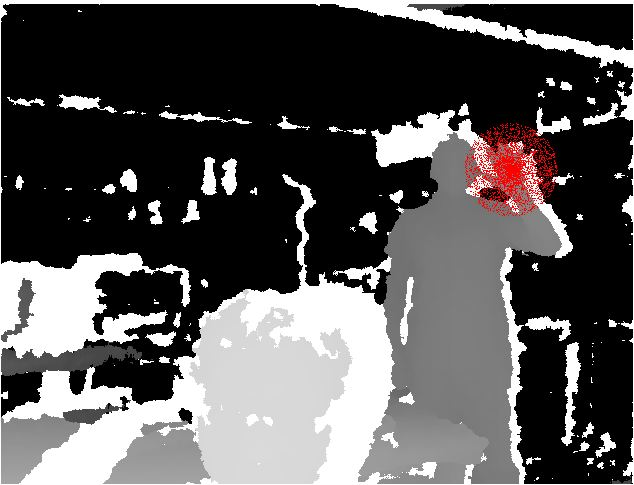
\includegraphics[width=0.23\textwidth]{fig/OpenHandFarOffset.jpg}
	
	\caption{Offset pairs for a given pixel. In the left figure, the reference pixel is the center of the palm. In the right figure, the reference pixel is the center of the palm of the person that stands. }
	\label{fig:offset}
\end{figure}

This feature extraction method is also used in \cite{shotton2011}. The offsets $\theta=\{\bf{u}, \bf{v} \}$ are generated randomly. In our design, we make those offsets to be uniformly sampled from a bounded circular area.  
$\textbf{u}$ and $\textbf{v}$ are obtained as
\begin{align}
\label{enq: offest}
 (r \cos \beta, r \sin \beta),
\end{align}
where $r$ and $\beta$ are uniform random variables:
\begin{align}
 r &= U[R_{\text{min}}, R_{\text{min}}] \\
 \beta &= U[0, 2\pi]
\end{align}

 As we can see from Figure \ref{fig:offset}, the offset pairs are located within the neighborhood of the palm and is adaptive to the depth.  
\todo{DO WE NEED MORE EXPLANATION?}

\subsection{The Classifier: SVM or Random Forest?}

In the training samples each pixel is labeled (we would deal with how to generate massive labeled sample in Section \ref{sec: generating_training}   and we have to use a supervised learning methods. Two methods come into our decision of choice: linear SVM and random forest. Let us make the notation as follows: the number of training samples: $l$, the number of features: $n$, the number of classes (types of gestures): $c$. Our main criteria for choosing the best algorithm are (1) prediction time and (2) accuracy. 

\textbf{Linear SVM.} In linear SVM, a model that is $c$ number of weight vector length of $n$ is trained. In prediction, the prediction is based on the dot product between the trained weight vectors and the feature vector. Therefore,  the run-time complexity for predicting each pixel is $O(n\times c)$.



\textbf{Random Forest.} Random forest is built on an ensemble of decision trees that are trained on a bootstrap the training samples. Each node in the decision tree has one feature and a threshold to determine which branch to go to. Without pruning the decision tree, the depth of the tree is approximately as $O(\log l)$. Therefore $O(\log l)$ queries of features are made in a single decision tree when prediction. The run-time complexity for random forest is then $O(\log l \times n_{\text{tree}})$. In fact, we can prune each decision tree to limit its depth. Pruning is also crucial for us since it can guarantee the worst-case prediction time. Moreover pruning can make the decision tree (which is a binary tree) almost balanced, ensuring the per-pixel prediction can proceed in an almost constant time.   [TO DO(how to prune)] Say the maximum depth is $d_{\text{tree}}$, the prediction complexity can go down to $O(d_{\text{tree}}\times n_{\text{tree}})$. 

\todo{Show RF algorithm}

\textbf{Comparison.} Let us do a simple calculation in which we use a realistic parameter setting. Suppose we have 2000 features, 3 classes, and using 3 trees with maximum depth of 20, the random forest is 100 times faster than linear SVM! Moreover, in our experimental evaluation, random forest has proven to be far superior than linear SVM in accuracy. Although linear SVM might use some advanced feature learning technique such as deep learning to achieve similar accuracy as to random forest, SVM is still too slow for us to adopt in the system. Inheriting from decision tree, random forest allows the system to extract features \textbf{on-demand}, which has been extremely crucial for real-time application as in the case of our system. The second author \todo{HOW ABOUT THE FIRST AUTHOR? He's never surprised} is really surprised by this analysis since he used to believe linear SVM is unbeatable in practice.  

\textbf{Training.} Training in linear SVM can be very fast as it can has a run-time complexity of $O(n\times l)$ and there exists technique to scale the training to distributed system \todo{Cite Michael's paper}. Training in random forest, however, does not have an optimization-based foundation. We use brute force to determine the right feature and right threshold for each node in the decision forest. In determining the right threshold, we use grid search. In the training of random forest, it is highly recommended to put the training data in the main memory. 


\subsubsection{GPU For Real-time Prediction} 
There are $307,200$ $(640\times 480)$ pixels in a frame. Each pixel will undertake $O(d_{\text{tree}}\times n_{\text{tree}})$ operations for prediction. We first tried to implement the random forest prediction using CPU. It takes about 1 minute to process a frame! GPU has to be used since it allows massive parallelism. As can be seen in Figure~\ref{fig: GPUvsCPU}, GPU is more suitable for high-parallelism and high-latency jobs, while CPU is better fit for low-parallelism and low-latency jobs. 

\begin{figure}
	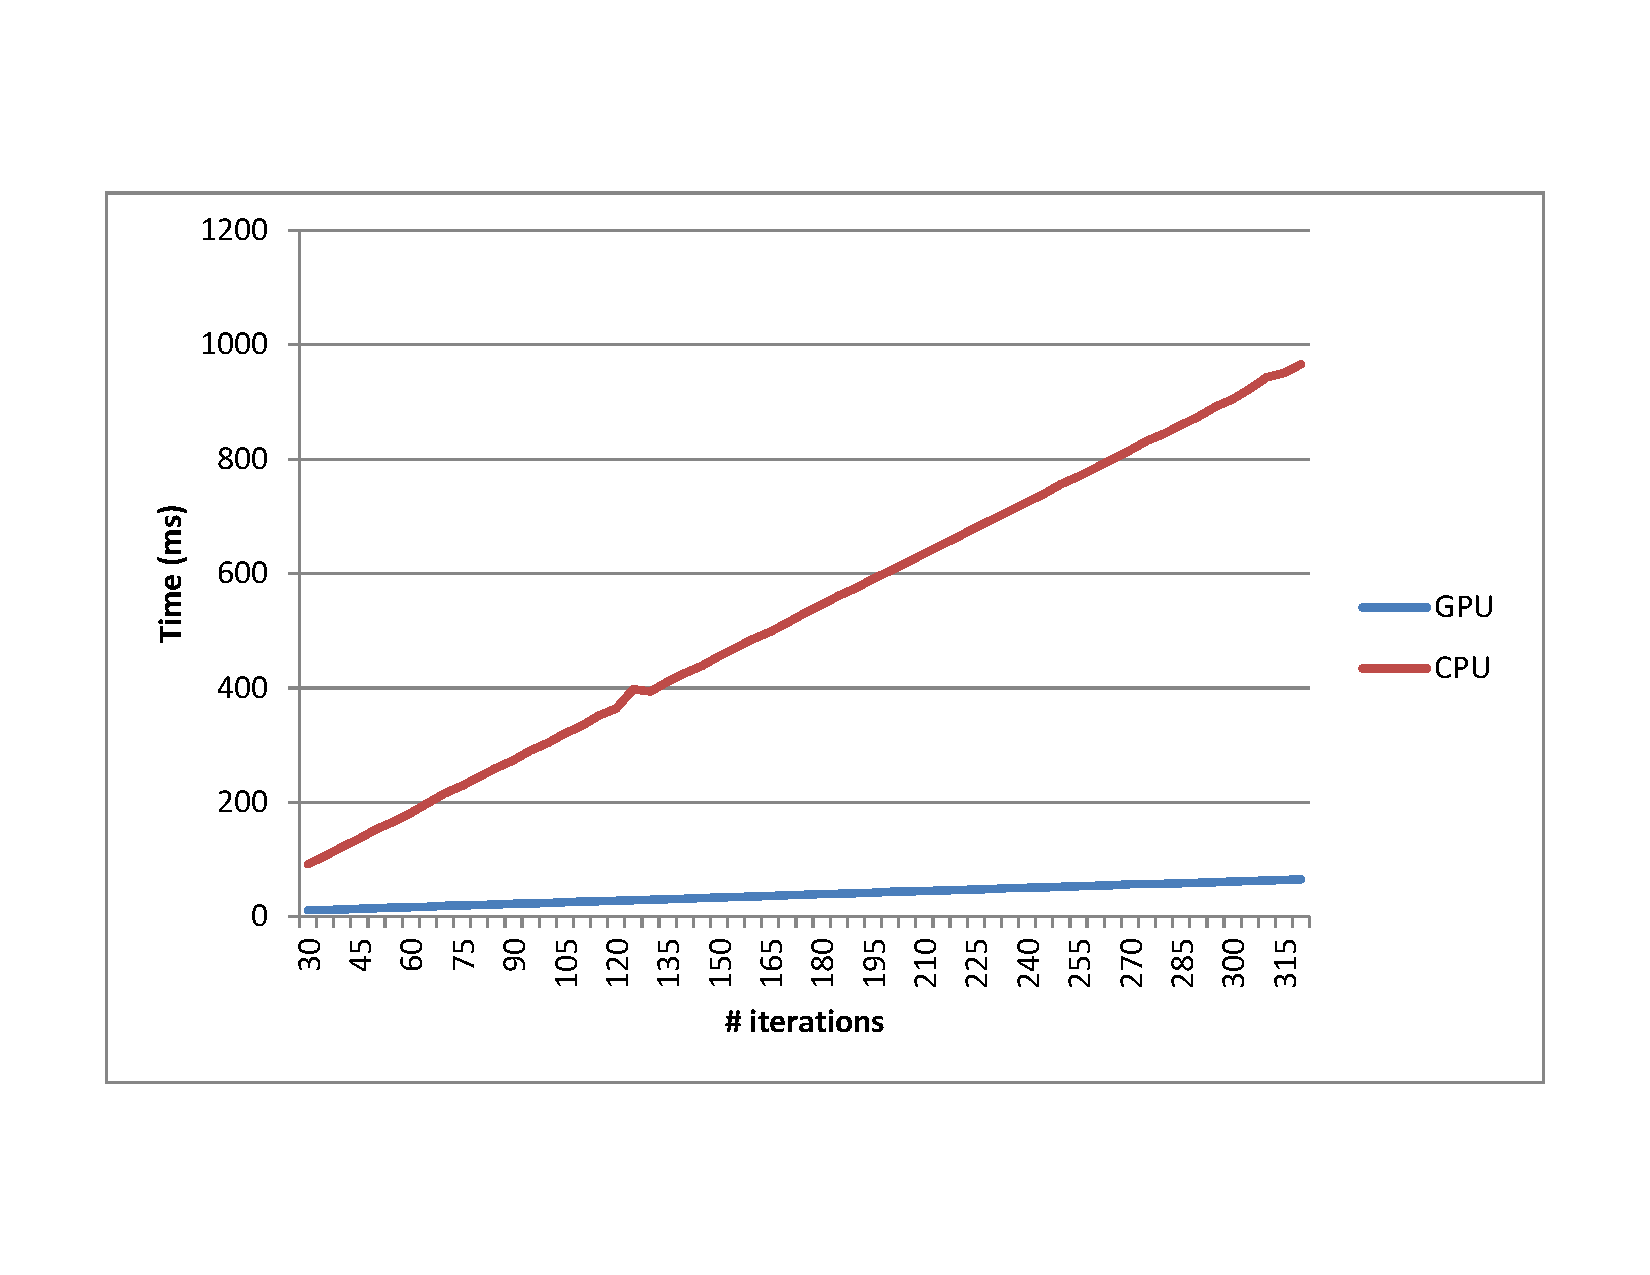
\includegraphics[width=0.45 \textwidth]{fig/GPUvsCPU.pdf}   
    \caption{A computational comparison between GPU and CPU. A simple experiment is conducted by varying the number of iterations in a for-loop. GPU would parallelize the for loop.}
    \label{fig: GPUvsCPU}
\end{figure}

In our system, each pixel has fired a thread to make prediction using random forest. In a typical GPU, more than thousands of threads are running concurrently thanks to the special architecture of GPU. As a result, per-pixel classification can be done in about 40ms \todo{Exact number}.    


\section{Pooling}
\label{sec: pooling}
\cutsection

After training on the labeled data sets and making per-pixel prediction, our system would take the per-pixel's predicted class as input and propose the final location and type of the gesture. We have considered several candidates. First we considered to use mean shift, a similar approach used in \todo{MSR}. However we found that the complexity of mean shift is very high: $O(N^2)$, where N is the number of pixels (in our case $N= 307200$). Then we consider to use clustering, i.e., unsupervised learning. The methodology is as follows: we treat non-background pixels (after per-pixel classification) all equally (without any labels) and then run clustering on them. Then we would use the largest cluster as a proposal of the hand and use the majority of the predicted label as the type of the gesture. The location of the gesture is found by the 2D median of the largest cluster to prevent outliers. In the choice of clustering algorithms, we consider bother K-means and density-based clustering.

\textbf{K-means.} K-means is probably the most commonly used clustering algorithm. A parameter K, the number of clusters, has to be specified beforehand. K-means is fast, with a complexity of $O(2N_{\text{non-background}})$, where $N_{\text{non-background}}$ is the number of non-background pixels. We found that however there is a significant weakness in the application of K-means to our system: (1) K-means assume each cluster has an equal size of points; and (2) K-means is not robust to outliers. As a result, K-means is very likely to divide a hand as two clusters. Therefore we abandon the use of K-means in our system.

\textbf{Density-based clustering.} Density-based cluster is more suitable for graphics application as it tries to cluster points that has a density exceeding pre-determine threshold. We customize the density-based clustering as in Algorithm \todo{DBScan algorithm}. The complexity is O($N_{\text{non-background} }\epsilon^2$), where $\epsilon$ is the radius of the interested pixels that is used in Algorithm 
\todo{DBScan algorithm}.

\begin{algorithm}[t]
%\vskip -0.1in
 \caption{Density-based clustering}
 
\begin{algorithmic}
 \State Input: a depth image with labeled pixels
   \For{each non-background and unvisted pixel $p$}

      \State mark $p$ as visited
         \State neighbor\textunderscore list $\gets$ get\textunderscore neighbors($p$, $\epsilon$ )
         \If{ len(neighbor\textunderscore list) $>$ $\epsilon^2 \times$ density }
            \State add $p$ to a new cluster
            \State create a queue: Seed
            \State enqueue neighbor\textunderscore list to Seed
            \While{Seed not empty}
                \State pixel $t$ $\gets$ Seed.Dequeue()
                \State neighbor\textunderscore list $\gets$ get\textunderscore neighbors($t$, $\epsilon$ )
                \If{len(neighbor\textunderscore list) $>$ $\epsilon^2 \times$ density }
                   \For{each pixel $q$ in neighbor\textunderscore list}
          \If{ $q$ is not visited}                    
                      \State Seed.Enqueue($q$)
                      \State mark $q$ as visited
                      \State add $q$ to the new cluster
                    \EndIf
                   \EndFor 
                \EndIf
            \EndWhile
         \EndIf

  \EndFor
\\
\Function{get\textunderscore neighbors}{$q$, $\epsilon$} 
	\State list is empty	
 	\For{each pixel $x$ that is within $\epsilon$ distance of $q$}
		\If{$x$ is labeled as non-background}
			\State add $x$ into list
		\EndIf 	
 	\EndFor  	
 	\\
 	\Return list
\EndFunction

\end{algorithmic}
\end{algorithm}





\section{Implementation}

There are several implementation details that worth mentioning here. 

\subsection{Kinect}
We have purchased two Kinect sensors: one for XBox the other for Windows. Kinect SDK is a Windows-based API allowing us to access the raw depth and RGB images from both versions of Kinect. The Windows version offers a near mode to permit objects to be within 30cm of the Kinect. In the labeling the color gloves to generate training samples, we use the built-in function provided by Kinect SDK to map the color pixel to depth pixel. The color detection turns out not to work very well since there are many noises due to lighting and the camera. However with cropping and depth-thresholding, we managed to labeled hundreds of images. At this time, we did not use the gloves with fingers colored, as we found (1) it is difficult to produce a perfectly built color gloves and (2) the low resolution of the Kinect sensor might not capture the details of figure very well.

\subsection{GPU Implementation}
From a programmer's perspective, GPU is seen as an I/O device: one has to move the data from main memory to the GPU memory and move back the processed data to the main memory. There are several libraries for us to consider to program on GPU: Microsoft DirectX, Microsoft DirectCompute, OpenCL, CUDA. We decided to use OpenCL as it is a standard library for general purpose computing on GPU and can run on almost all GPU (as opposed on CUDA which can only run on NVidia cards). OpenCL is using C as the programming language and has an event-queue framework to process incoming data. 

We have considered the layout of the decision tree in the GPU memory since we found the cache hit is low. We have tested (1) recursively root-> left sub-tree and then right sub-tree, and (2) breath first data structures. It turns out there is no significant difference between the two data structures. So we use the first data structure.  

\subsection{Training}
* EC2
* Virtual wall
* Changing double to float saves a lot of space


\textbf{Actual System.}
* Use C$^\sharp$ and C++
* Show actual system picture here



\section{Experimental results}
\label{sec: experiments}

% Bigger picture
There are many parameters involved in capturing the training images, extracting features, and training the random forest classifier. To study the contribution of these parameters, we systematically varied them and studied the accuracy of the resulting classifier. To study the accuracy, we set aside a collection of images as the test set and trained on a different set of images. We didn't use cross-validation due to the time constraints in training a random forest; it would have taken considerably longer time to test the cross validation accuracy and would  have prevented us from running as many tests as we did.

% Parameters tested
\subsection{Experiments}
We collected images of four different gestures shown in figure~\ref{fig:gestures}. We refer to each image that we captured as a ``training sample''. Since there are over 300000 pixels in each image, we sampled only 2000 of them so that we can train on more diverse images. From each image, we sampled 1000 background points, and 1000 points from the gesture to ensure we trained evenly on the different types of classes.

\textbf{Varying Parameters.} We varied three parameters in training the models. We varied the number of trees in the forest from two trees to five trees; 1000, 2000 and 3000 features; and different number of training images starting at 10, 50, 100 up to 350 increments of 50. We also set aside 50 images as the test set. For each of these 96 configurations, we trained a random forest model and computed the test set accuracy.

The features represent randomly selected offsets from the point of prediction. The offsets are radially sampled up to a maximum radius. We varied the radius of the sampling and generated feature files. We trained models with 2000 features, three trees, and different number of training images for radii set to 20, 40, 60, 100 and 200. \todo{WHAT UNIT IS THIS??? - mmpx. Explain this.}

Based on the results, we varied the parameters more in interesting directions: (1) We studied the effect of training a forest with just one tree, (2) we trained with 689 training images and 100 test images, and (3) we tried smaller radii for the feature offsets. 

In addition to varying the parameters, we conducted four more experiments. 

\textbf{Randomness.} First, due to the nature of the random forest, the trained model is non-deterministic and may yield a different accuracy rate for the same training set of images. In order to study this randomness, we trained ten models on the the same training set with 1000 features, 300 training images, and one tree. 

\textbf{SVM Comparison.} Second, we compared random forest classifier with a linear SVM classifier. We trained an SVM classifier for 2000 features, and different number of training images. 

\textbf{Pruning.} Third, we studied the effect of pruning on the accuracy of prediction. To study this, we pruned the forests trained with 2000 features and three trees for different number of training images. Then we calculated the test set accuracy of the pruned models.

\textbf{Overfitting.} Finally, we studied how much the model overfits to the training samples by calculating the training accuracy and comparing that with the test accuracy. We fixed 2000 features and three trees and varied the number of training samples. 

We used the ALGLIB \cite{alglib} for the random forest implementation, and LIBLINEAR \cite{liblinear} for SVM implementation.

\subsection{Results}

\begin{figure}
\begin{center}
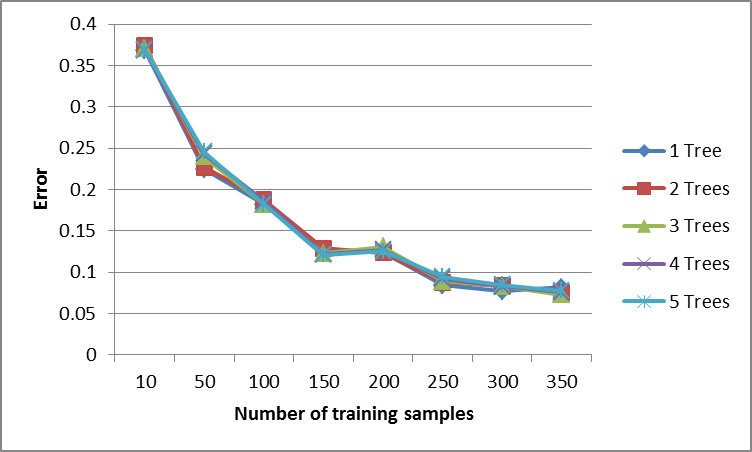
\includegraphics[width=0.45 \textwidth]{fig/varytrees.png}
\end{center}
\caption{We trained a classifiers with 2000 features, 350 training images and varied the number of trees from 1 to 8. The error is reported on a test set of 50 images.}
\label{fig:varytrees}
\end{figure}

\begin{figure}
\begin{center}
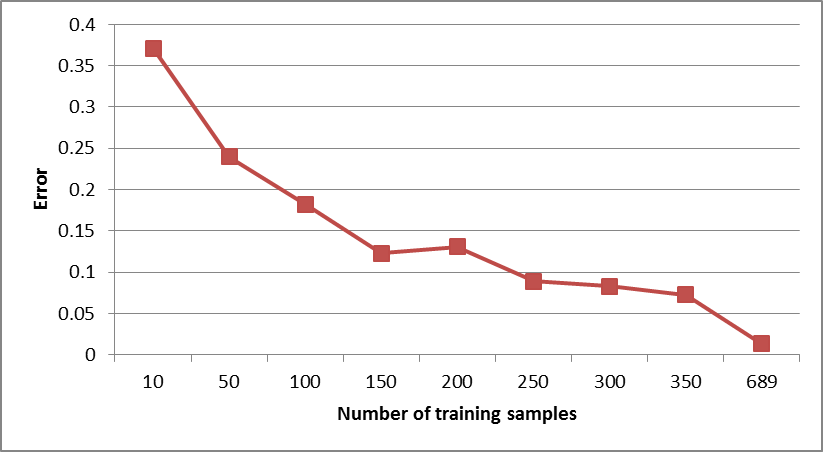
\includegraphics[width=0.45 \textwidth]{fig/largetraining.png}
\end{center}
\caption{We fixed the number of features at 2000, and the number of trees at 3 and varied the number of training images. Except for the last experiment, the error is reported on a test set of 50 images. Due to the size of the last training set, we increased the test set to 100 images.}
\label{fig:largetraining}
\end{figure}

\begin{figure}
\begin{center}
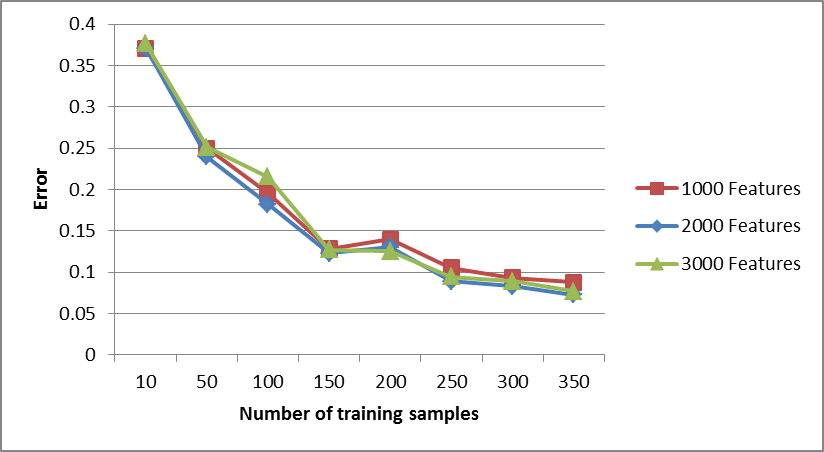
\includegraphics[width=0.45 \textwidth]{fig/varyfeatures.png}
\end{center}
\caption{We varied the number of features with three trees, and 350 training samples.}
\label{fig:varyfeatures}
\end{figure}


\begin{figure}
\begin{center}
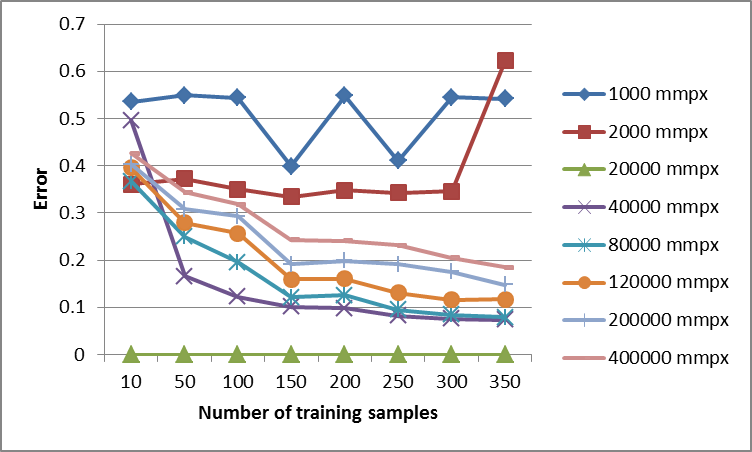
\includegraphics[width=0.45 \textwidth]{fig/varyradii.png}
\end{center}
\caption{We varied the maximum radius of the offsets used in generating the feature vectors. We fixed the number of features to 2000, and number of trees to 3.}
\label{fig:varyradii}
\end{figure}

\textbf{Varying Parameters.} Figure~\ref{fig:varytrees} shows the results of varying the number of trees while fixing the remaining parameters. We observed that the number of trees makes no noticeable difference. In fact, even training the forest with one tree has the same accuracy as the with multiple trees. This was also observed for different fixed values of the parameters. Adding multiple trees in the random forest is intended to protect against overfitting. However, our test and training sets were sampled from the same pool of images so we hypothesize one tree is sufficient to model all the variability in the test set. 

Figure~\ref{fig:largetraining} shows the effect of varying the number of training samples. There is a clear trend of smaller test error as we increase the number of training samples. At 689 training samples, the error is only 1.32\%. Increasing the number of training samples had the biggest impact in reducing the error when compared to other factors. 

Figure~\ref{fig:varyfeatures} shows the effect of varying the number features. Across most of our experiments we observed that using 2000 features outperforms 3000 features, which outperforms 1000 features. However, as seen in figure~\ref{fig:varyfeatures}, the difference in error is small. This suggests that if we sampled 1000, 2000, and 3000 features again, we may observe a different trend.

Finally, figure~\ref{fig:varyradii} shows the results of varying the radius of the offset features. For smaller training sample sizes, setting the radius to 40000 mmpx gives the least error classifier. However, as we increase the number of training samples, both 40000 mmpx and 80000 mmpx give similarly accurate classifiers. This means that when we have fewer training samples, setting the radius to 40000 mmpx will allow us to train a more accurate classifier, but when we have many training samples, the radius is not so important. We notice that making the radius too small or too large gives poor accuracy. By qualitatively checking the offset images as shown in figure~\ref{fig:offset}, we hypothesize that to train a more accurate classifier, the offsets should cover most of the hand, and then some of the background. If the radius is too small, then the offsets will be right next to each other and feature vectors for different gestures may be too similar.

\textbf{Randomness.} Training 10 models with the same parameters, we got a mean error of 9.82\% with 0.94\% standard deviation. The randomness is training the random forest is very concentrated around the mean. \todo{More? Or just leave this out?}


\begin{figure}
\begin{center}
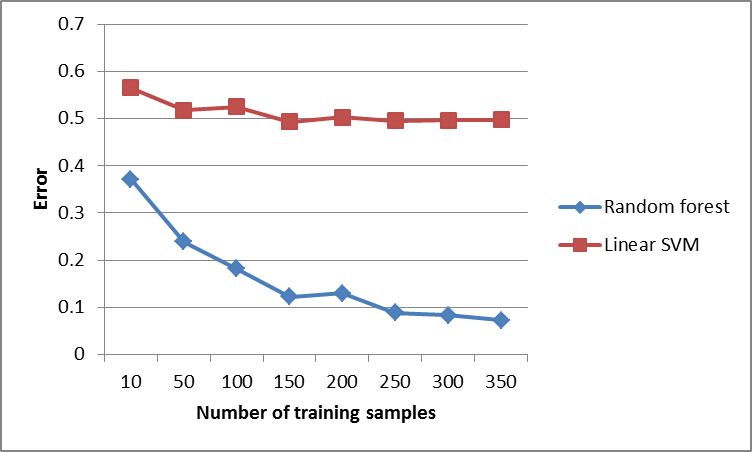
\includegraphics[width=0.45 \textwidth]{fig/linearsvm.png}
\end{center}
\caption{Using 2000 features, and 350 training images we trained a linear SVM and a random forest. The random forest was trained with 3 trees.}
\label{fig:linearsvm}
\end{figure}


\textbf{SVM Comparison.} Figure~\ref{fig:linearsvm} compares the error rate of a linear SVM with a random forest classifier. Linear SVM only slightly outperforms a random classifier that always predicts a pixel as the background. As we increase the training sample size, linear SVM improves much more slowly than the random forest.

\textbf{Pruning.} Pruning the tree showed almost no difference in accuracy compared to the full tree. We hypothesize the reason for this is that very high up in the tree the splitting nodes already confidently divide the training points into their class. However, ALGLIB continues to exhaust the features until the entire tree is constructed. By stopping the prediction early on in the tree, we don't suffer in accuracy, and improve the speed of prediction.

\begin{figure}
\begin{center}
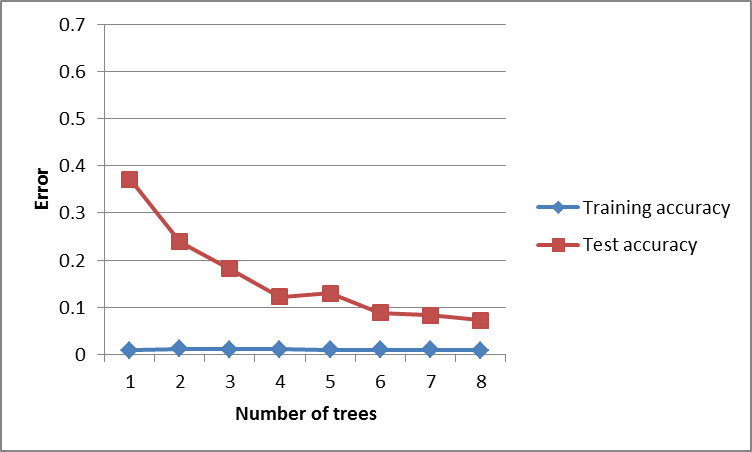
\includegraphics[width=0.45 \textwidth]{fig/trainingacc.png}
\end{center}
\caption{We fixed the number of features at 2000 and the number of trees at 3. For each training sample size, we compare the training accuracy and the test accuracy.}
\label{fig:trainingacc}
\end{figure}

\textbf{Overfitting.} Figure~\ref{fig:trainingacc} shows evidence of extreme overfitting. The training error is consistently very low (mean 1.06\%) and is much lower than the testing accuracy. 





\section{Experience}
\subsection{Limitations}
Our current system is not without limitations. First, the real-time prediction component cannot achieve a frame rate at 30Hz but at about 5Hz.

\section{Related Work}

There are two main techniques in hand gesture recognition - appearance based and model based. These are akin to probabilistic models of classification and generative models of classification respectively. \textbf{Appearance based} approaches read the pixels from the camera and build classifiers to label that as belonging to a finite set of classes. The main limitation of this technique is that the set of labels is finite and fixed ahead of time. The advantage of appearance based approaches is their implementation is often extremely fast and therefore suited for situations where live classification is important. Examples of appearance based techniques can be found in \cite{shotton2011, wang2009}. \textbf{Model based} approaches start with a set of hypotheses of the final classification based on rules of the object being classified. For instance, in the case of hand gestures a hypothesis can be a particular orientation of the joints.  An advantage here is that the hypotheses can be generated from an infinite space of possible classifications. The main disadvantage of model-based techniques is that they are often computationally expensive. In addition, model-based approaches tend to be very complex. An example of a model based technique can be found in \cite{oikonomidis2011}.

As advance sensor technology has become more accessible, many developers and researchers are studying natural interfaces. \cite{stuerzlinger2010} overviews a variety of input devices for interfacing with 3D models including mouse designs with six degrees of freedom, haptics devices for simulating realistic forces, and computer vision based techniques for head and hand tracking. Very relevant to our project, \cite{hoffman2010} presents a method for identifying 25 gestures in 3D using the gyroscope and accelerometer in the Nintendo Wii remote. This falls in a more general category called ``spatially convenient input-devices''. 

The work most similar to ours is from Microsoft \cite{shotton2011} on the details of the Kinect's appearance-based skeleton recognition algorithm. They classify each pixel as belonging to some portion of the body and then pool all pixels from each portion to determine the joint positions. Their training set is generated from synthetic 3D images of body orientations. The feature extraction technique and the random forest classification algorithm used in this work is borrowed from \cite{lepetit2005}. Our project differs from this in the method for generating training samples, and the scale of classification. 

\cite{wang2009} present another appearance-based method for detecting hand gestures using just an RGB camera. Their solution requires the user wear a glove with a special pattern imprinted on it. The camera pictures the hand in different orientations, normalizes the image, and identifies the nearest neighbor in a database of common hand gestures. Unlike this approach, our technique only uses a color glove for training purposes. 

\cite{oikonomidis2011} present a model-based approach using the Kinect. They first generate a set of hypotheses with knowledge of inverse kinematics, and approximate shape of fingers and hands. They evaluate these hypotheses and pick the most likely one based on the depth image from the Kinect. This technique is able to detect hand gestures even in the place of occlusions and is implemented efficiently reaching up to 15 updates per second. However, being model-based, this technique may be vulnerable to differences in hand shapes, and still lags behind in speed compared to appearance-based techniques. 

\section{Conclusion}

\bibliographystyle{unsrt}
\begin{thebibliography}{9}

\bibitem{shotton2011} J. Shotton, A. Fitzgibbon, M. Cook, T. Sharp, M. Finocchio, R. Moore, A. Kipman, A. Blake. Real-time human pose recognition in parts from single depth images. CVPR, 2011.

\bibitem{wang2009} R. Wang and J. Popovi\'c. Real-time hand-tracking with a color glove. In Proc. ACM SIGGRAPH, 2009.

\bibitem{oikonomidis2011} I. Oikonomidis, N. Kyriazis, and A. Argyros. Efficient model-based 3D tracking of hand articulations using kinect. In BMVC, Aug 2011.

\bibitem{lepetit2005} V. Lepetit, P. Lagger, and P. Fua. Randomized trees for real-time keypoint recognition. In Proc. CVPR, pages 2:775-781, 2005. 

\bibitem{liblinear} R.-E. Fan, K.-W. Chang, C.-J. Hsieh, X.-R. Wang, and C.-J. Lin. LIBLINEAR: A library for large linear classification Journal of Machine Learning Research 9(2008), 1871-1874.

\bibitem{schneiderman1996} B. Schneiderman. The eyes have it: a task by data type taxonomy for information visualizations. Visual Languages, 1996.

\bibitem{keim2002} D.A. Keim. Information visualization and visual data mining. Visualization and Computer Graphics, IEEE Transactions. Vol 8, no.1, pp. 1-8, Jan 2002.

\bibitem{stuerzlinger2010} W. Stuerzlinger, C Wingrave. The value of constraints for 3D user interfaces. Dagstuhl Seminar on VR, 2010.

\bibitem{hoffman2010} M. Hoffman, P. Varcholik, and J. LaViola. Breaking the status quo: improving 3D gesture recognition with spatially convenient input devices. IEEE VR, 2010.

\bibitem{alglib} V. Bystritsky. ALGLIB. 14 Aug 1999. Web. \url{http://www.alglib.net}.

\end{thebibliography}

\end{document}
